\section{Stand der Technik}

\lipsum[1][1-5]

\subsection{Überschrift Ebene 2}

\lipsum[1][1-7] \cite{web:webseite1}

\subsection{Überschrift Ebene 2}

\lipsum[1][1-3]

\begin{equation} \label{glg:1}
    F=m \cdot a
\end{equation}

In Gleichung \ref{glg:1}  ist der Zusammenhang von Kraft F zu Masse m und Erdbeschleunigung
g in bekannter Weise dargestellt.

\subsubsection{Überschrift Ebene 3}

Lorem ipsum dolor sit amet, consectetur adipisici elit, sed eiusmod tempor incidunt ut labore
et dolore magna aliqua \cite{publikation:publikationtitel2}.Ut enim ad minim veniam, quis nostrud exercitation ullamco
laboris nisi ut aliquid ex ea commodi consequat, siehe Abbildung \ref{fig:Bild2}.

In Gleichung \ref{glg:2} ist der Zusammenhang von elektrischer Spannung U als das Produkt von
ohmschem Widerstand R und elektrischer Stromstärke I als Ohmsches Gesetz dargestellt.

\begin{align}
    U & = R \cdot I \label{glg:2}                    \\
    P & = U \cdot I \cdot \cos \varphi \label{glg:3}
\end{align}

Die elektrische Leistung P ergibt sich laut Gleichung \ref{glg:3} aus dem Produkt der elektrischen
Spannung U, der elektrischen Stromstärke I und dem Leistungsfaktor \(\cos \varphi\).

\begin{figure}[H]
    \centering
    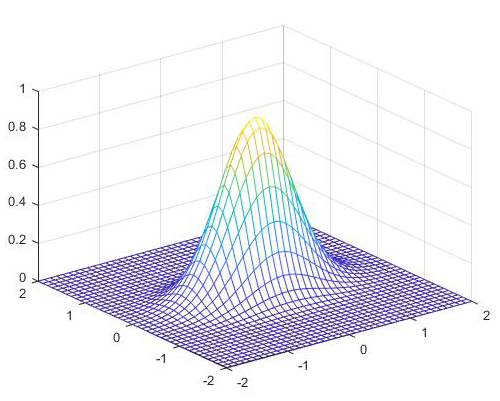
\includegraphics[scale=0.9]{20_Hauptteil/20_Dateien/Bild2.png}
    \caption{Beschriftung der übernommenen Abbildung \cite{web:webseite1}.}
    \label{fig:Bild2}
\end{figure}

\subsubsection{Überschrift Ebene 3}

Lorem ipsum dolor sit amet \cite{zeitschrift:zeitschrifttitel1}, consectetuer adipiscing elit. Ut purus elit, vestibulum ut,
placerat ac, adipiscing vitae, felis.

\begin{quote}
    \textit{\lipsum[2][1-5]}
\end{quote}

\lipsum[1][1-3]

\subsubsection{Überschrift Ebene 3}

\lipsum[1][1-15]

\subsection{Überschrift Ebene 2}

\lipsum[1][1-9]
Excepteur sint obcaecat cupiditat non proident, sunt \SI{10}{\micro\second}
in culpa qui \ac{mrk} officia deserunt mollit \ac{ros} anim id est laborum \cite{datasheet:can}.

In Tabelle \ref{tab:Tabelle1} ist eine Übersicht der wichtigsten Parameter der
Robotik-Realisierungen entsprechend dem Stand der Technik als Gegenüberstellung dargestellt.

\begin{table}[H]
    \centering
    \setlength{\arrayrulewidth}{0.1mm}
    \setlength{\tabcolsep}{13pt}
    \renewcommand{\arraystretch}{1.8}
    \begin{tabular}{ |p{4cm}|c|c|c|c|c| }
        \hline
        Robotik Realisierung & A\cite{publikation:publikationtitel1} & B\cite{publikation:publikationtitel2} & C\cite{buch:buchtitel1} & D\cite{zeitschrift:zeitschrifttitel1} & E\cite{web:webseite1} \\
        \hline
        Dynamik [m/s]        & 7,87                                  & 1530                                  & 11,7                    & 10,3                                  & 6,51                  \\
        Freiheitsgrade [1]   & 19,32                                 & 164                                   & 14,2                    & 45,2                                  & 3,98                  \\
        Genauigkeit [mm]     & 8,90                                  & 15                                    & 12,3                    & 0,1                                   & 6,58                  \\
        Masse [kg]           & 8,96                                  & 1083                                  & 16,2                    & 60,0                                  & 0,01                  \\
        Kosten               & gering                                & mittel                                & hoch                    & gering                                & mittel                \\
        \hline
    \end{tabular}
    \caption{Übersicht der Robotik-Realisierungen entsprechend dem Stand der Technik.}
    \label{tab:Tabelle1}
\end{table}